\chapter{Desarrollo hardware del manipulador}
\label{cap:capitulo5}

\vspace{1cm}

En este capítulo se aborda el desarrollo necesario para, a partir de un concepto, acabar construyendo un prototipo real funcional. Se 
hace incisión en cada etapa necesaria para este cometido.


Escribe aquí un párrafo explicando brevemente lo que vas a contar en este capítulo. En este capítulo (y quizás alguno más) es donde, por fin, describes detalladamente qué has hecho y qué experimentos has llevado a cabo para validar tus desarrollos.

\section{Concepto}
En esta sección se expone como ha sido el proceso de encontrar y definir la idea fundamental del robot, en función de 
los objetivos propuestos, evaluando las distintas opciones para encontrar el que mejor se adapte. Se trata de balance

Primero, se debe conocer el numero de grados de libertad que se ajuste a los requisitos establecidos en la sección \ref{sec:requisitos}. En base 
a los requisitos 1 y 5, que limitan en cuanto a precio de fabricación y complejidad de los mismos, se ha decidido limitar los grados de 
libertad a un máximo de 4. 

hablamos del tipo de joints que existente

Con 4 grados de libertad vamos mal pero se puede.
Tipos:
Scara

RR

Basado en paralelos

\section{Modelo alámbrico}
\subsection{En qué consiste}
\label{subsec:eqc_mod_alambrico}
El modelo alámbrico es una forma de analizar el movimiento de un sistema mecánico compuesto por ejes y eslabones. Este 
enfoque simplifica la representación visual al destacar las relaciones espaciales entre las diferentes partes del sistema mediante 
líneas y conexiones simbólicas, en lugar de mostrar detalles realistas del manipulador. 
\begin{figure} [h!]
  \begin{center}
    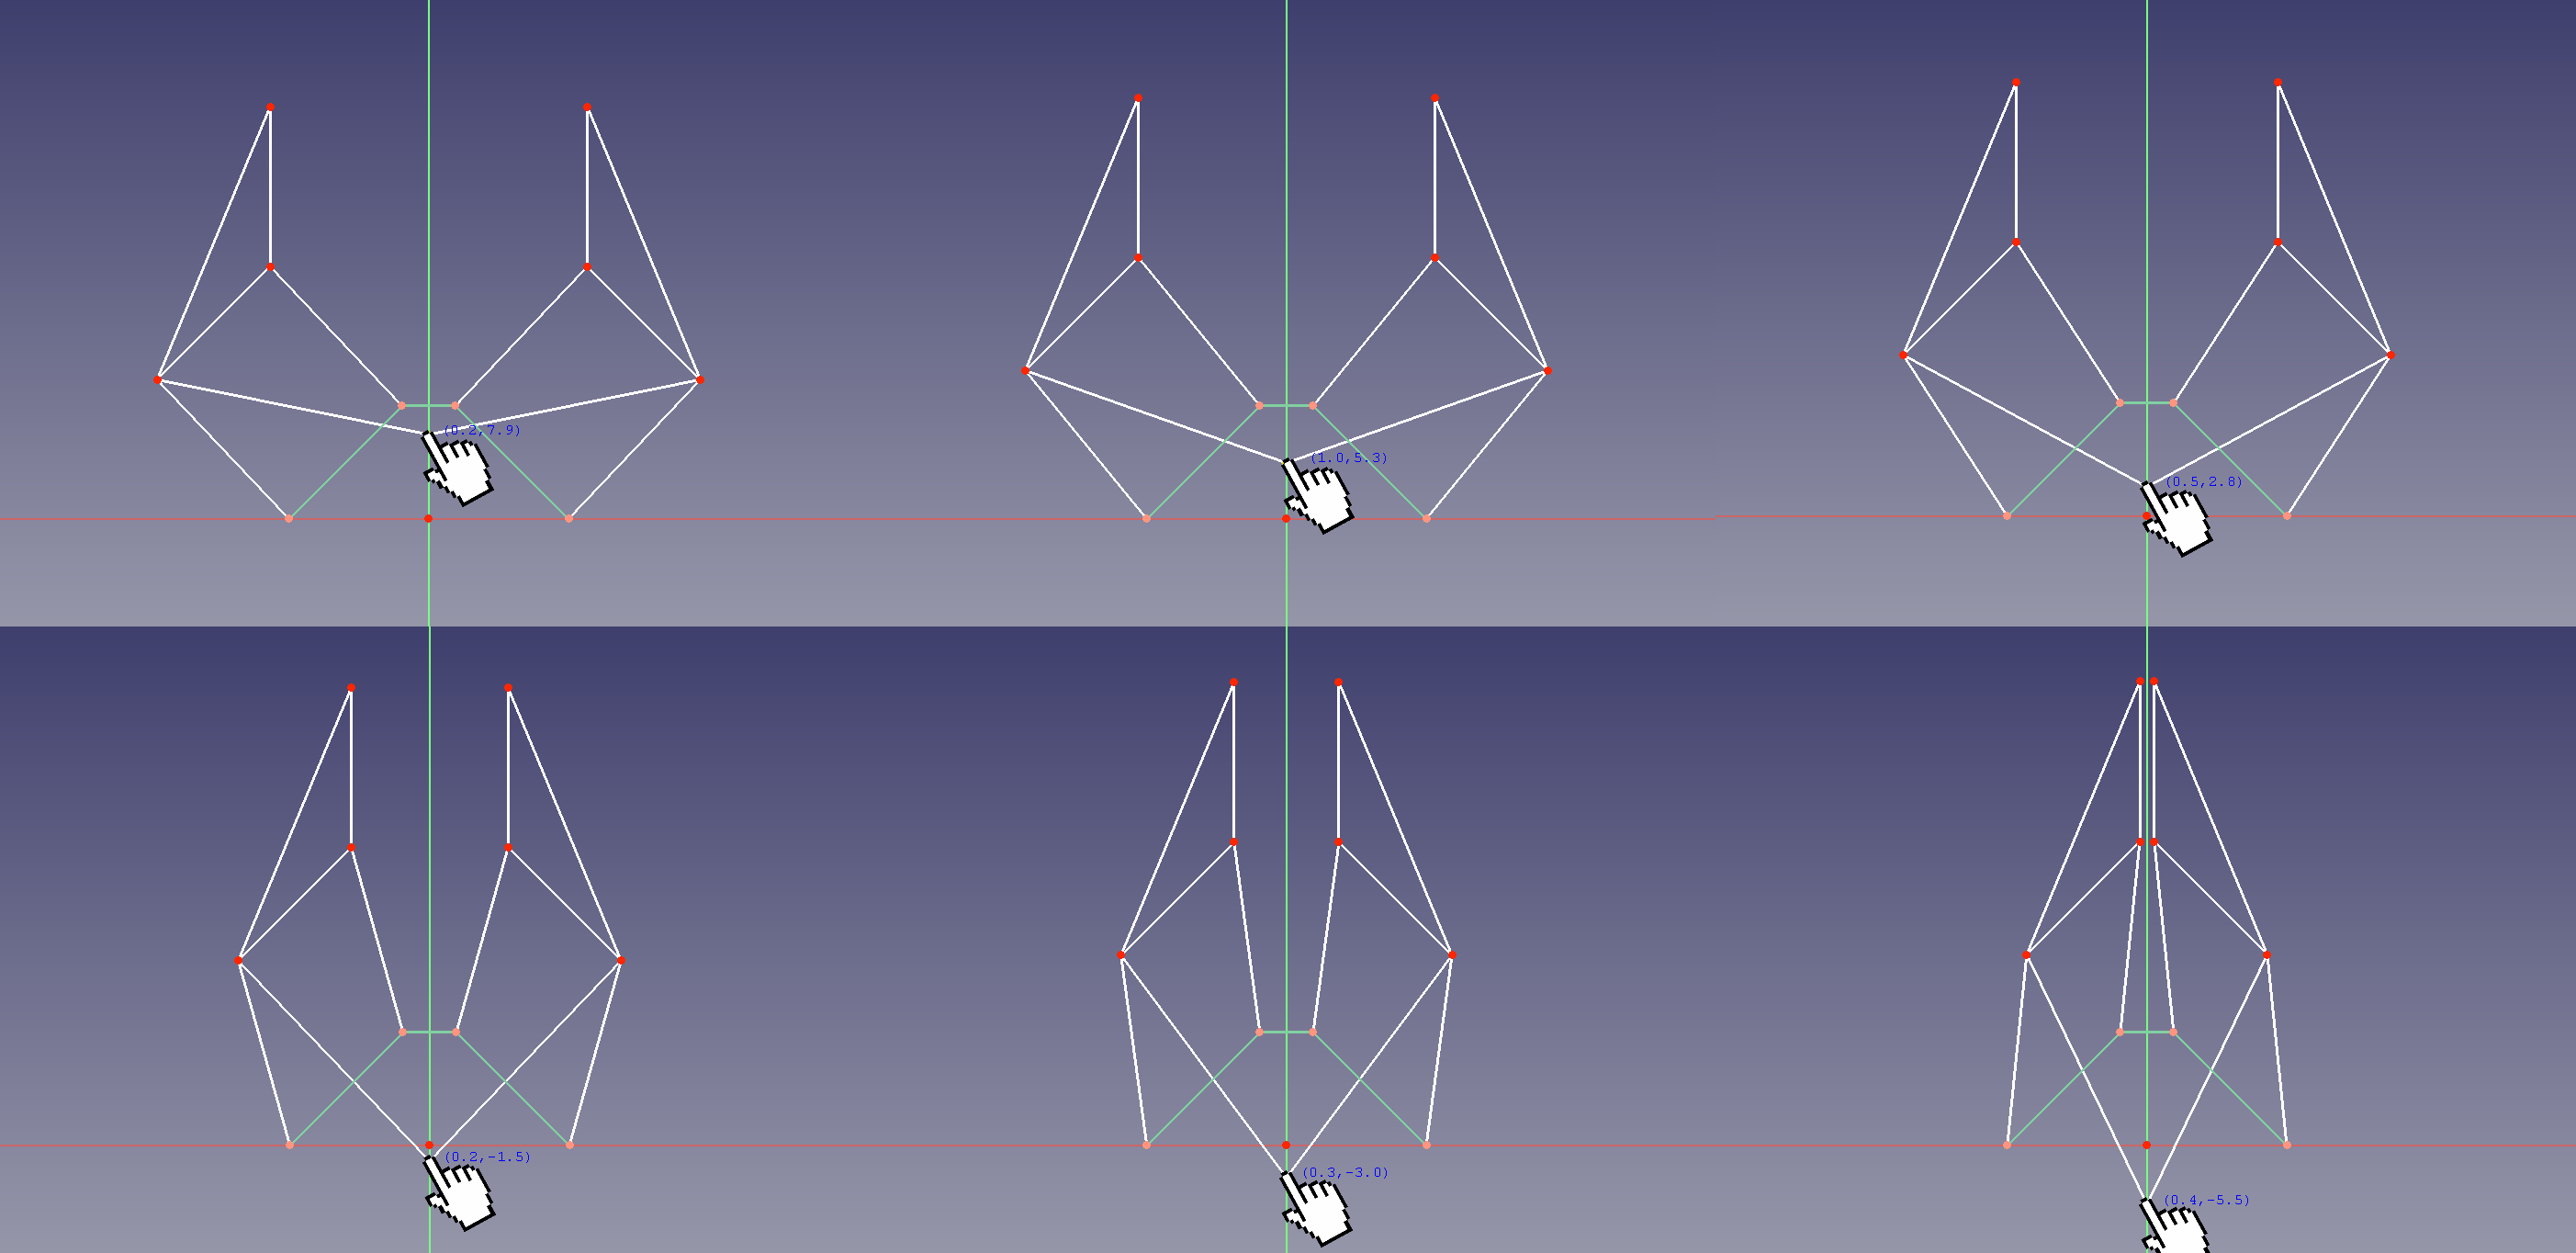
\includegraphics[width=15cm]{figs/pinza_evol.png}
  \end{center}
  \caption{Pinza paralela con 1 grado de libertad}
  \label{fig:mod_pinza_figure}
\end{figure}\ 

\subsection{Modelo alámbrico del brazo MeArm \ref{fig:mearm}}
\label{subsec:mod_mearm}


\section{Dinámica}

\section{DH}

\section{Bocetos}

\section{Diseño CAD}

\section{Diseño CAD}


\begin{code}[h]
\begin{lstlisting}[language=C++]
void Memory::hypothesizeParallelograms () {
  for(it1 = this->controller->segmentMemory.begin(); it1++) {
    squareFound = false; it2 = it1; it2++;
    while ((it2 != this->controller->segmentMemory.end()) && (!squareFound)) {
      if (geometry::haveACommonVertex((*it1),(*it2),&square)) {
        dist1 = geometry::distanceBetweenPoints3D ((*it1).start, (*it1).end);
        dist2 = geometry::distanceBetweenPoints3D ((*it2).start, (*it2).end);
      }
    // [...]
\end{lstlisting}
\caption[Función para buscar elementos 3D en la imagen]{Función para buscar elementos 3D en la imagen}
\label{cod:codejemplo}
\end{code}

En el Código \ref{cod:codejemplo2} vemos un ejemplo escrito en \texttt{Python}.

\begin{code}[h]
\begin{lstlisting}[language=Python]
def mostrarValores():
    print (w1.get(), w2.get())

master = Tk()
w1 = Scale(master, from_=0, to=42)
w1.pack()
w2 = Scale(master, from_=0, to=200, orient=HORIZONTAL)
w2.pack()
Button(master, text='Show', command=mostrarValores).pack()

mainloop()
\end{lstlisting}
\caption[Cómo usar un Slider]{Cómo usar un Slider}
\label{cod:codejemplo2}
\end{code}

\section{Verbatim}

Para mencionar identificadores usados en el código ---como nombres de funciones o variables--- en el texto, usa el entorno literal o verbatim \verb|hypothesizeParallelograms()|. También se puede usar este entorno para varias líneas, como se ve a continuación:

\begin{verbatim}
void Memory::hypothesizeParallelograms () {
  // add your code here
}
\end{verbatim}

\section{Ecuaciones}

Si necesitas insertar alguna ecuación, puedes hacerlo. Al igual que las figuras, no te olvides de referenciarlas. A continuación se exponen algunas ecuaciones de ejemplo: Ecuación \ref{ec:ec1} y Ecuación \ref{ec:ec2}.

\begin{myequation}[h]
\begin{equation}
H = 1 - \frac{\sum_{i=0}^{N}\frac{(\frac{d_{j_s} + d_{j_e}}{2})}{N}}{M}
\nonumber
\label{ec:ec1}
\end{equation}
\caption[Ejemplo de ecuación con fracciones]{Ejemplo de ecuación con fracciones}
\end{myequation} 

\begin{myequation}[h]
\begin{equation}
v(entrada)= \left\{
	\begin{array}{lcc}
		0 & \mbox{if} & \epsilon_t < 0.1\\
		K_p\cdot{(T_{t}-T)} & \mbox{if}& 0.1 \leq \epsilon_t < M_t\\
		K_p \cdot M_t & \mbox{if}& M_t < \epsilon_t
	\end{array}
\right.
\label{ec:ec2}
\end{equation}
\caption[Ejemplo de ecuación con array y letras y símbolos especiales]{Ejemplo de ecuación con array y letras y símbolos especiales}
\end{myequation}

\section{Tablas o cuadros}

Si necesitas insertar una tabla, hazlo dígnamente usando las propias tablas de \LaTeX, no usando pantallazos e insertándolas como figuras... En el Cuadro \ref{cuadro:ejemplo} vemos un ejemplo.

\begin{table}[H]
\begin{center}
\begin{tabular}{|c|c|}
\hline
\textbf{Parámetros} & \textbf{Valores} \\
\hline
Tipo de sensor & Sony IMX219PQ[7] CMOS 8-Mpx \\
Tamaño del sensor & 3.674 x 2.760 mm (1/4" format) \\
Número de pixels & 3280 x 2464 (active pixels) \\
Tamaño de pixel & 1.12 x 1.12 um \\
Lente & f=3.04 mm, f/2.0 \\
Ángulo de visión & 62.2 x 48.8 degrees \\
Lente SLR equivalente & 29 mm \\
\hline
\end{tabular}
\caption{Parámetros intrínsecos de la cámara}
\label{cuadro:ejemplo}
\end{center}
\end{table}

